\section{Theorie}
\label{sec:Theorie}
Ziel dieses Versuches ist es mithilfe verschiedener Brückenschaltunge unbekannte Widerstände, Kapazitäten und Induktivitäten zu bestimmen.
Außerdem soll das Verhalten der Brückenspannung in Abhängigkeit von der Frequenz mithilfe der Wien-Robinson-Brücke untersucht werden.

\subsection{Allgemein}
\label{subsec:allgemein}
Eine Brückenschaltung ist eine bestimmte Verschaltung von verschiedenen elektrischen Bauelementen, sie hat allgemein die in \autoref{fig:brücke} dargestellte Form.

\begin{figure}[H]
    \centering
    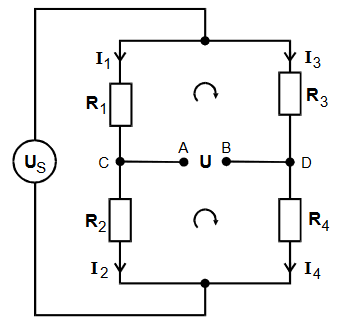
\includegraphics[height=4cm]{build/allgemein.PNG}
    \caption{Allgemeine Form einer Brückenschaltung.\cite[216]{V302}}
    \label{fig:brücke}
\end{figure}

\noindent Innerhalb der Schaltung wird zwischen zwei Punkten eine Potentialdifferenz in Abhängigkeit von den vorliegenden Widerstandsverhältnissen analysiert.
Dies Potentialdifferenz wird auch als Brückenspannung bezeichnet.
Die Grundlage für die mathematischen Berechnungen sind die zwei Kirchhoffschen Gesetze.\\
Das erste Gesetz ist die Knotenregel

\begin{equation}
    \sum_k I_k = 0 .
    \label{eqn:knoten}
\end{equation}

\begin{figure}[H]
    \centering
    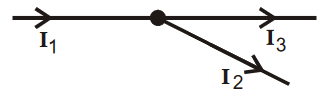
\includegraphics[width=0.2\textwidth]{build/knoten.PNG}
    \caption{Graphische Darstellung der Knotenregel.\cite[217]{V302}}
    \label{fig:knoten}
\end{figure}

\noindent Sie besagt, dass in einem Verzweigungspunkt die Summe aller zufließenden elektrischen Ströme gleich der Summe der abfließenden elektrischen Ströme ist. 
Das zweite Gesetz ist auch bekannt als die Maschenregel

\begin{equation}
    \sum_k E_k = \sum_k I_k R_k.
    \label{eqn:masche}
\end{equation}

\begin{figure}[H]
    \centering
    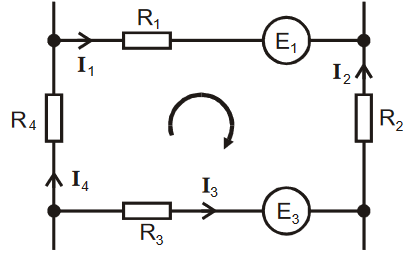
\includegraphics[width=0.3\textwidth]{build/maschen.PNG}
    \caption{Graphische Darstellung der Maschenregel.\cite[217]{V302}}
    \label{fig:maschen}
\end{figure}

\noindent Nach diesem ist in einem in sich geschlossenem Stromkreis bzw. einer geschlossenen Masche die Summe der Spannungen gleich null. 
Dabei ist das Vorzeichen der einzelnen Summanden positiv, wenn die Stromrichtung vom betrachteten Bauteil mit dem Uhrzeigersinn läuft.\\
Sobald in der Brückenschaltung Kapazitäten $C$ und Induktivitäten $L$ zusätzlich zu ohmschen Widerstänenden $R$ enthalten sind, muss mit Impedanzen gerechnet werden.
Dies ist zurückzuführen auf den Blind- und Wirkwiderstand eines Kondensators bzw. einer Spule.
Die Widerstandsoperatoren sind 

\begin{align}
    Z_C &= -\frac{j}{\omega} C , & Z_L &= j\omega L  &\text{und}& &Z_R = R .
    \label{eqn:operatoren}
\end{align}

Ein spezieller Fall einer Brückenschaltung ist die abgeglichene Brücke, wo die Brückenspannung unabhängig von der anliegenden Speisepannung verschwindet, wenn 
\begin{equation}
    Z_1 Z_4 = Z_2 Z_3
    \label{eqn:abgleichbed}
\end{equation}
gilt.\\
Die folgenden Brückenschaltungen sind Beispiele für abgeglichene Brücken.

\subsection{Wheatstonesche Brücke}
\label{subsec:wheatstone}

\begin{figure}[H]
    \centering
    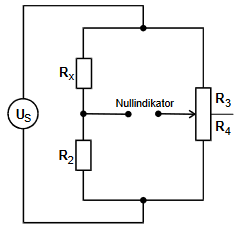
\includegraphics[width=0.3\textwidth]{build/wheat.PNG}
    \caption{Schaltbild der wheatstoneschen Brücke.\cite[219]{V302}}
    \label{fig:wheat}
\end{figure}

Diese Schaltung besteht nur aus ohmschen Widerständen und wird zu Bestimmung eines unbekannten Widerstand $R_x$ verwendet.
Durch Anwendung der Kirchhoffschengesetze folgt für den unbekannten Widerstand

\begin{equation}
    R_x = R_2 \frac{R_3}{R_4}.
    \label{eqn:wheat}
\end{equation}

Für $R_3$ und $R_4$ wird ein Potentiometer benutzt, weil die Abgleichbedingung nur vom Verhältnis der beiden Widerstände anbhängig ist und nicht von deren Größe.

\subsection{Kapazitätsmessbrücke}
\label{subsec:kapazitäts}

\begin{figure}[H]
    \centering
    \includegraphics[width=0.3\textwidth]{build/kapazität.PNG}
    \caption{Schaltbild der Kapazitätsmessbrücke.\cite[220]{V302}}
    \label{fig:kapazität}
\end{figure}

Die Wärmeverluste des realen Kondensators werden in der Schaltung durch einen (fiktiven) ohmschen Widerstand berücksichtigt, der mit der Kapazität in Reihe geschaltet wird.
Im Gegensatz zu der Wheatstoneschen Brücke werden somit zwei unbekannte Größen bestimmt $C_x$ und $R_x$.
Außerdem wird noch eine weitere bekannte Kapazität $C_2$ eingebaut und $R_2$ ist nun ein veränderbarer Widerstand.
Der Widerstandsoperator hat die Form

\begin{equation}
    Z_{C_{real}} = R - \frac{j}{\omega C}
    \label{eqn:widerop_kap}
\end{equation}

dadurch gilt für die Kapazität

\begin{equation}
    C_x = C_2 \frac{R_4}{R_3}
    \label{eqn:kapazität_kap}
\end{equation}

und für den Widerstand

\begin{equation}
    R_x = R_2 \frac{R_3}{R_4}
    \label{eqn:widerstand_kap}
\end{equation}

Bei manchen Kondensatoren sind die dielektrischen Verluste so gering, dass der (fiktive) ohmsche Widerstand gegen null geht, somit gilt $R_2 \approx 0$.


\subsection{Induktivitätsmessbrücke}
\label{subsec:induktivität}

\begin{figure}[H]
    \centering
    \includegraphics[width=0.3\textwidth]{build/induktivität.PNG}
    \caption{Schaltbild der Induktivitätsmessbrücke.\cite[221]{V302}}
    \label{fig:induktivität}
\end{figure}

Diese Schaltung ähnelt der Kapazitätsmessbrücke mit dem einzigen Unterschied, dass anstelle von Kapazitäten nun Induktivitäten verwendet werden.
Auch bei der Induktivitätsmessbrücke gibt es Wärmeverluste, aufgrund der magnetischen Feldenergie.
Deswegen wird ein (fiktiver) ohmscher Widerstand mit der Induktivität in Reihe geschaltet.
Der Widerstandsoperator wird abgebildet durch

\begin{equation}
    Z_{L_{real}} = R + j\omega L
    \label{eqn:widerop_ind}
\end{equation}

Die Abgleichbedingung für die Induktivität ist

\begin{equation}
    L_x = L_2 \frac{R_3}{R_4}
    \label{eqn:induktivität_ind}
\end{equation}

und für den Widerstand gilt

\begin{equation}
    R_x = R_2 \frac{R_3}{R_4}
    \label{eqn:widerstand_ind}
\end{equation}

Die Spule mit der bekannten Induktivität $L_2$ sollte möglichst geringe Verluste besitzen, da diese sonst die Ergebnisse verfälschen. 
Deswegen wird häufig eine andere Brückenschaltung zur Bestimmung der Induktivität benutzt.
Zum Beispiel die Maxwell-Brücke, die im folgenden näher beschrieben wird.

\subsection{Maxwell Brücke}
\label{subsec:maxwell}

\begin{figure}[H]
    \centering
    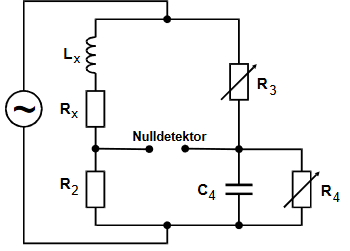
\includegraphics[width=0.3\textwidth]{build/maxwell.PNG}
    \caption{Schaltbild der Maxwell Brücke.\cite[222]{V302}}
    \label{fig:maxwell}
\end{figure}

Anstelle einer bekannten Induktivität wird in dieser Schaltung eine bekannte Kapazität $C_4$ mit geringen Verlusten genutzt.
Der Aufbau ist in \autoref{fig:maxwell} dargestellt.
Die verstellbaren $R_3$ und $R_4$ werden nun in Reihe und parallel zu $C_4$ geschaltet.
Außerdem ist $R_2$ nun ein fester bekannter Widerstand.
Die Widerstandsoperatoren sind

\begin{align}
    Z_1 &= R_x + j\omega L_x & \text{und}&  &\frac{1}{Z_4}=\frac{1}{R_4}+j\omega C_4
    \label{eqn:widerop_max}
\end{align}

Daraus folgt

\begin{equation}
    L_x = R_2 R_3 C_4
    \label{eqn:induktivität_max}
\end{equation}

für die Induktivität und für Widerstand

\begin{equation}
    R_x = R_2 \frac{R_3}{R_4}
    \label{eqn:widerstand_max}
\end{equation}

\subsection{Wien-Robinson-Brücke}
\label{subsec:wien-robinson}

\begin{figure}[H]
    \centering
    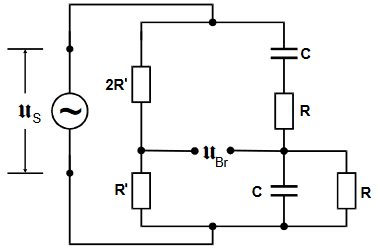
\includegraphics[width=0.3\textwidth]{build/wien-robinson.PNG}
    \caption{Schaltbild der Wien-Robinson-Brücke.\cite[222]{V302}}
    \label{fig:wien-robinson}
\end{figure}

Im Gegensatz zu den anderen Brückenschaltungen ist diese nur bei bestimmten Frequenzen abgleichbar.
Die Schaltung enthält nur bekannte Größen, die möglichst geringe Verluste und Tolernzen besitzen.
Sie besteht nur aus festen ohmschen Widerständen und Kapazitäten.
Die Wien-Robinson-Brücke ist eine Bandsperre und somit ein elektronischer Frequenzfilter.
Eine Bandsperre schwächt ein bestimmtes Frequenzband um die Grenzfrequenz
%Formel nü_0=w_0/2pi=1/cR2pi
\begin{equation}
    \nu_0 = \frac{\omega_0}{2\pi} = \frac{1}{CR2\pi}
    \label{eqn:grenzfrequenz}
\end{equation}

ab und lässt diese nicht passieren.
Die Übertragung lässt sich berechenen aus dem Spannungsverhätnis von Brückenspannung und Speisepannung
%f(omega)=Formel 19 in wurzelform
mit 
%omega gleich nü/Nü_0
Die Brückenspannung verschwindet bei 
\begin{equation}
    \omega_0 = \frac{1}{RC}.
\end{equation}
Eine Sinusschwingung sollte keine Oberwellen enthalten. 
Der Klirrfaktor gibt den Anteil der Oberwellen im Verhältnis zur Grundwelle einer Sinusschwingung an.
Die Kleinheit des Klirrfaktors
\begin{equation}
    k =  \sqrt{} siehe 228
\end{equation}
ist dementsprechend ein Maß für die Qualität eines Sinusgenerators.
Mitsamt der Annahme, dass die Summe der Oberwellen nur aus der zweiten Oberwelle besteht, lässt sich dies zu 
\begin{equation}
    k = \frac{U_2}{U_1}
    \label{eqn:keinf}
\end{equation}
vereinfachen.
Die Zweite Oberwelle wird bestimmt durch
%letzte Formel.

